%Notas sobre la definición del espectro.
\section{Qué es esto}
Un template de archivos .tex básico para escribir un texto sencillo.
Como podrá notar, separo en dos archivos .tex 
(``paquetes'' y ``estilo'')
los paquetes necesarios
para las ejecuciones así como el formato del documento.
Creo que así queda todo mucho más limpio. \\

Este es el template que usé para escribir mi tesis de licenciatura,
y que estoy adoptando para escribir todas mis notas. Me gusta mucho
tener un espacio amplio en el margen, en el que puedo escribir notas
e incluso agregar imágenes.

\begin{marginfigure}
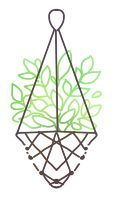
\includegraphics[scale= 1]{plant.jpg} 
\end{marginfigure}


\section{TODO}
Cuando tenga tiempo, voy a recopilar en este template
algunas expresiones útiles para mí, como lo son el 
poder poner imágenes en los márgenes o escribir
tablas en formatos que me gustan.
